\section{Modelling}
As mentioned earlier, we wish to model a framework of games instead of one
specific one, in order to encapsulate as many parameters as possible. The
simulation will have two factions, henceforth known as the town and the mafia.
The town wins when they have eliminated all mafia members. The mafia wins when
their factions have the non-strict numerical majority of players. The game is
played out in rounds consisting of four phases, which happen in order, until
either win-condition is met, as shown on figure \ref{fig:GameOverview}.
\begin{figure}[H]
	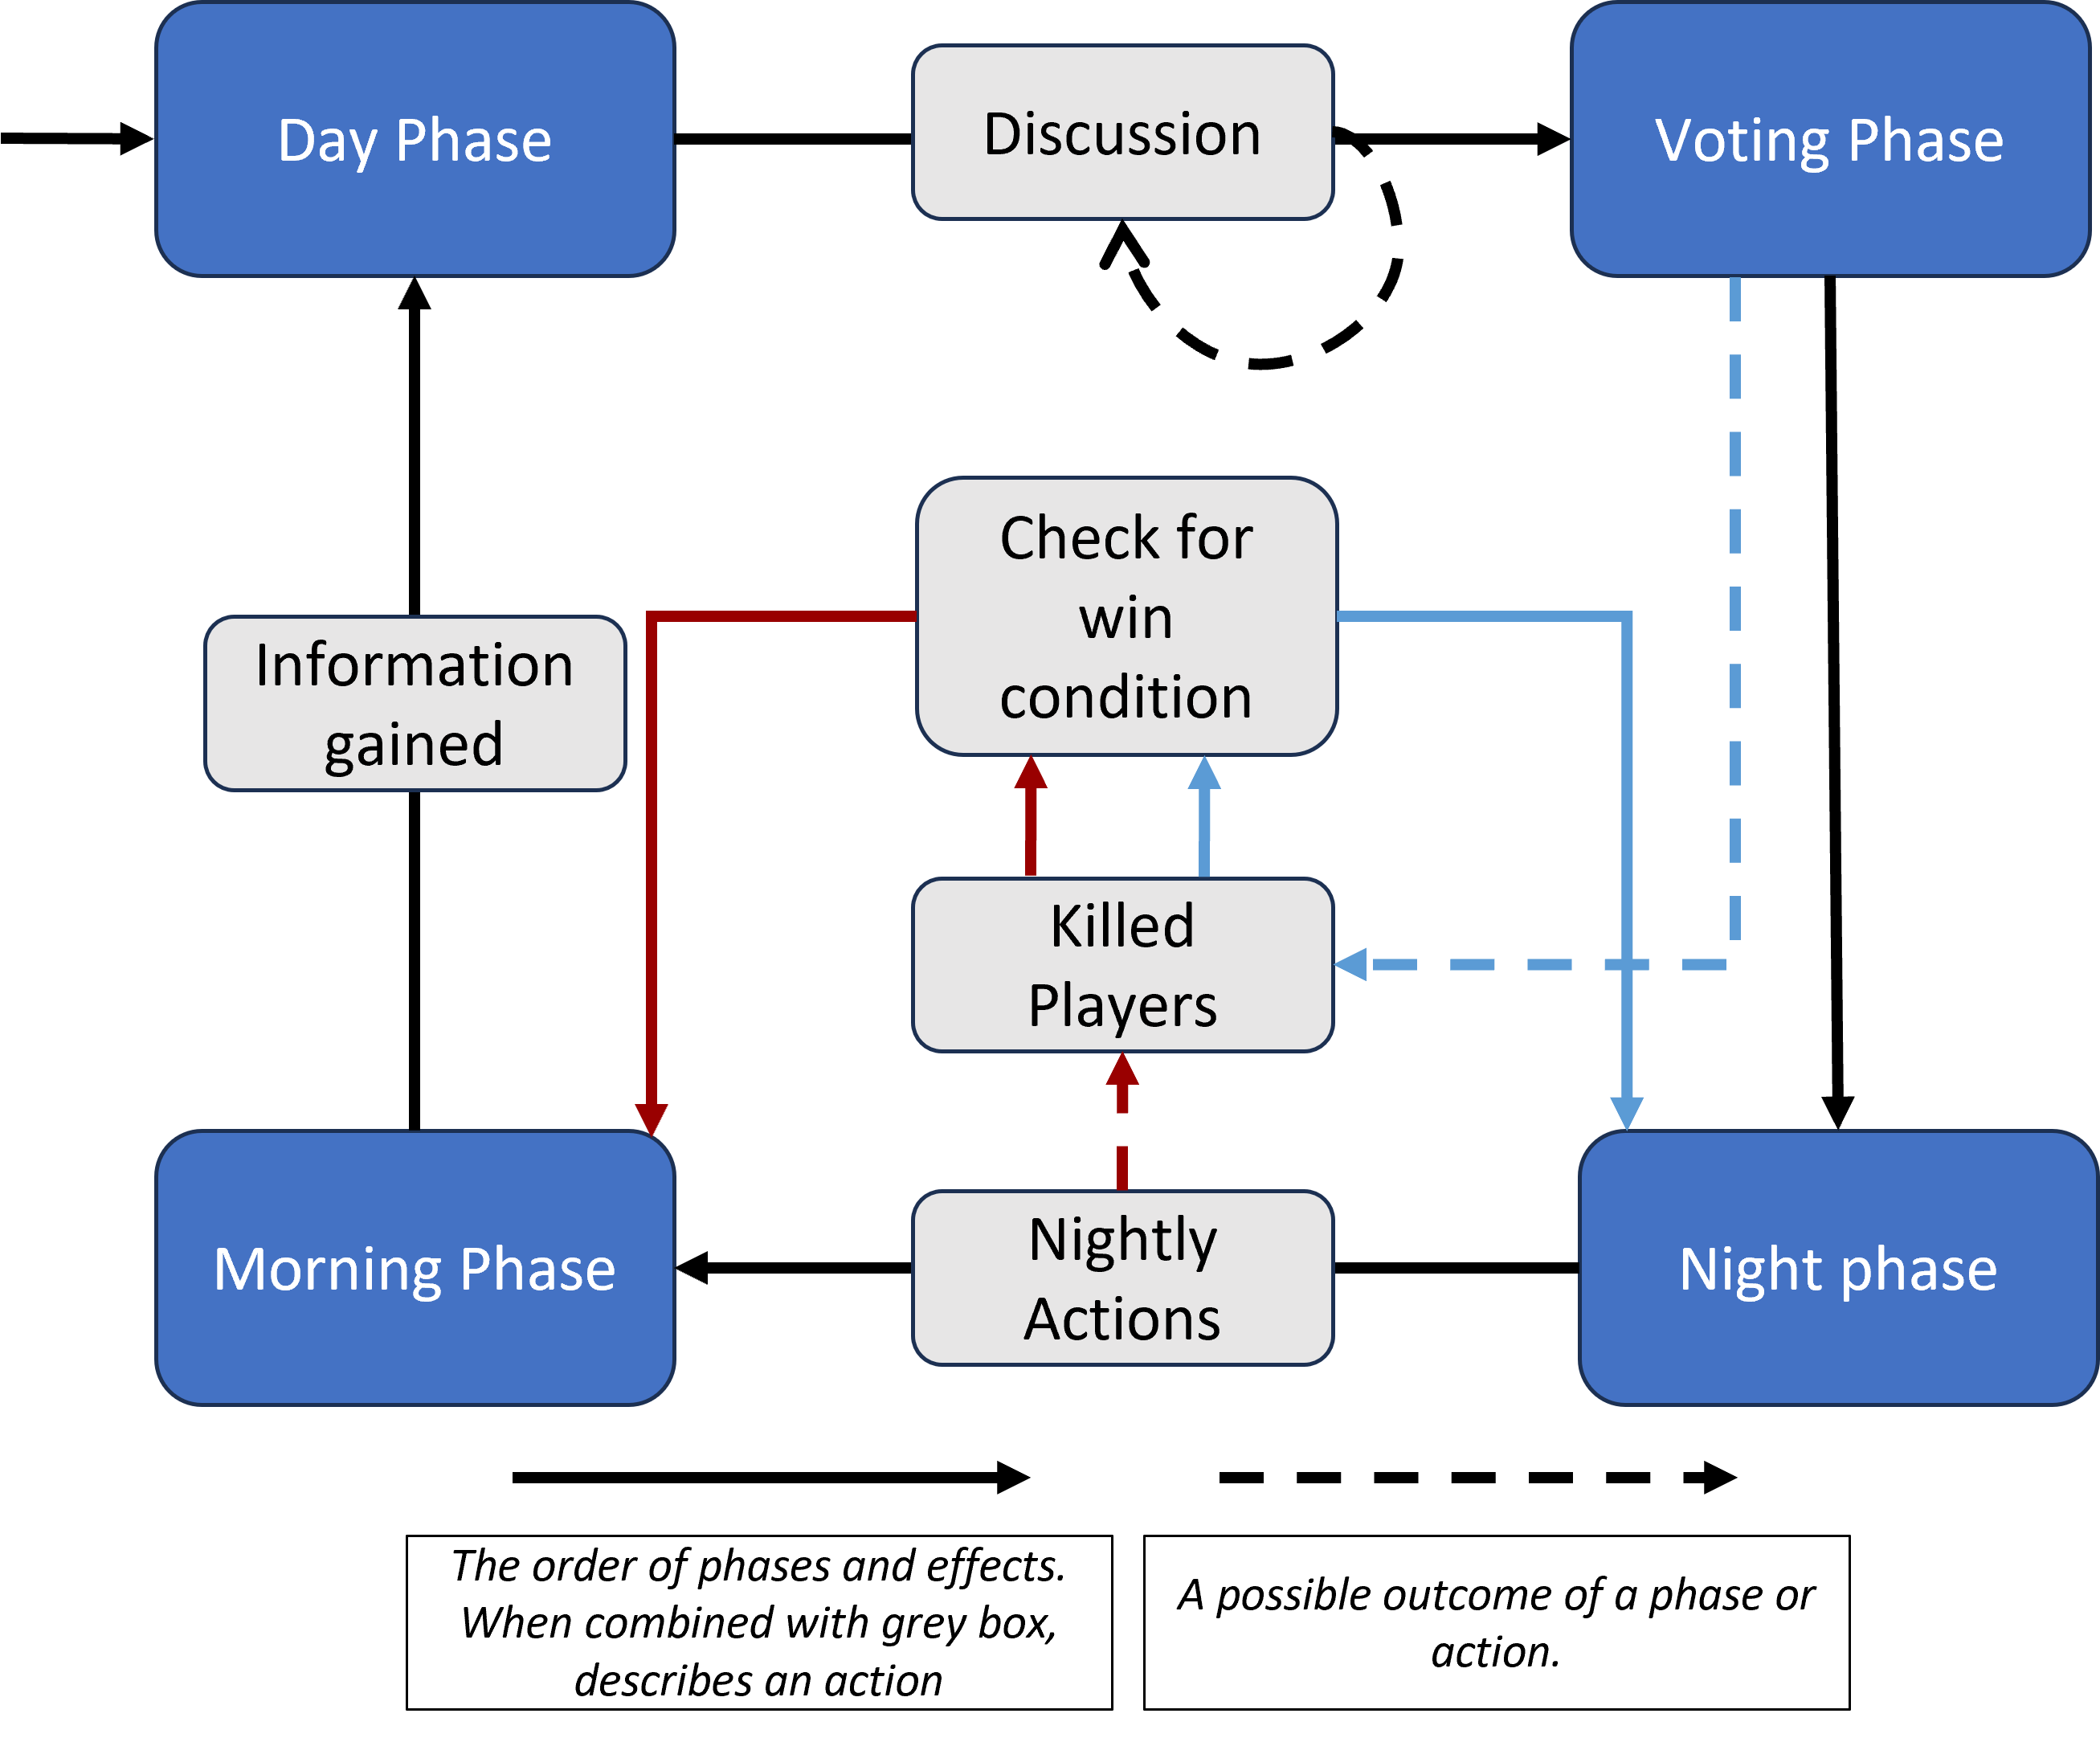
\includegraphics[width=1\linewidth]{figures/Game_overview3}
	\caption{Depicting the general flow of social deduction games. The blue arrows relate to the outcome of the voting phase. The red arrows relate to the outcome of the nightly actions}
	\label{fig:GameOverview}
\end{figure}

The night phase is where different roles perform private or public actions to
gain information or spread misinformation. The morning phase is where public
results of the night phase are revealed to all players. The roles of players
who died during the night phase is revealed at this time. The day phase is
where players try to influence each other's world views through communicative
actions. The voting phase is where players vote on who to lynch according to
their individual world views. The voting phase can end in a majority vote which
will result in a lynching of that player, killing them and revealing their role
publicly. It can also result in a tie, which will result in the phase ending
with no lynching.

In typical games, the most numerous role would be the villager who has no
special powers. However, as this paper wishes to analyse how the mafia can even
the odds against a town populated by special roles, they will not be used
extensively here. While all roles are explained in appendix \ref{app:A}, the
ones allied to the mafia, are covered below:

\begin{enumerate}
	\itemsep0px
	\item\textbf{Godfather} must choose one player each night to be eliminated.
	\item\textbf{Mafioso} performs the elimination on the godfathers' behalf. \todo{Context to elimination}
	\item\textbf{Consigliere} must choose one player each night and privately
	      gain information regarding their role.
	\item\textbf{Consort} must choose one player each night and prevent them
	      from performing any actions during the night phase.
	\item\textbf{Blackmailer} must choose one player each night to blackmail. A
	      blackmailed player can not communicate during the next day phase
	      \label{lst:Roles}
\end{enumerate}

Now, to simulate the games as closely as possible to the real world, we use a
foundation built upon a numerical approach to decision-making, and an
epistemological approach to the acquisition and updating of
knowledge\cite{commitment}. Their core principles are that players keep track
of all possible worlds that may be possible based on their own knowledge, and
the public knowledge available to them. They keep track of beliefs and lies by
'marking' worlds which contradict statements made by other players. Since there
should always be more players belonging to the town than the mafia, and that
the players of the town have no reason to lie, it is presumed that the world
with fewest 'marks' must be the true world. This is what the players will base
their decisions on. A few modifications to their methodology have been made, in
order to better suit a multi-round game \cite{commitment}.

First, the communicative actions for the game have been altered slightly. In
this simulation, players can choose between 5 different communicative actions:
\begin{enumerate}
	\itemsep0px
	\item \label{Com}Claim to have a certain role.
	\item Claim that someone else has a certain role.
	\item Inquire another player regarding their role.
	\item Inquire another player regarding their beliefs about other players.
	\item Do not say anything. \label{lst:communicativeActions}
\end{enumerate}
The purpose of these actions are to mimic the in-person game as closely as
possible. Players will each be able to take up to 3 communicative actions\footnote{The player can communicate 3 times but can choose not to communicate with the "Do not say anything" action\ref{lst:communicativeActions}} before the
phase concludes. Players choose which communicative actions to take, based on which communicative action
will provide the most information regarding their believed most likely world.

When public information is revealed, such as the role of a killed player, all
players must update their world views, eliminating all worlds not in accordance
with this information. This will iteratively limit the possible worlds,
granting more information to the players. The marks generated by communicative
actions are associated with the player that generated them. This means that
whenever public information is revealed about that player, players may either
discard or reinforce said marks. If the player was revealed to be a member of
the mafia, meaning that may have had incentive to lie players may choose to
discard the marks associated with that player. If they were a town member,
meaning they should have only told the truth other players may choose to
reinforce those marks.

Besides marks players keep track of active and inactive worlds. An active world
is a world that is true based on the public and private information available
to a player. An inactive world is a world that is true based on the public
information available, but false based on the private information available.
The need for inactive worlds, is that a player cannot assume that other players
are aware of private information, so these worlds must be included when
deciding which communicative actions to perform during the day phase.An
example:

Player 1 is a sheriff\footnote{A role allied to the town, who functions
	similarly to the consigliere}, and has used their nightly action to look at the
faction of player 2, which gave them the private information that player 2's
faction is of the town. Player 1 can now de-active all worlds where player 2 is
part of the mafia, as they are factually false. However, since this is not
public information player 1 knows that not everyone knows this, and these
worlds must therefore still be considered when choosing communicative actions,
even if just for knowing which worlds to avoid promoting. \\\\ Social deduction
scenarios can be expressed or modelled differently depending on the methods
used to solve them. While other noteworthy fields such as machine learning
could be used, we see an intriguing similarity between epistemology and social
deduction, which lies in the nature how these games are played. Often it's a
game between players henceforth called agents, who need to keep track of who
said what, who knows what, and what these truths entail. In the next section,
we will formalize such a model, based on dynamic epistemology and interrogative
inquiry, allowing agents to model their world view based on both facts and
communicative actions.